\documentclass[11pt,a4paper]{article}
\usepackage[T1]{fontenc}
\usepackage[utf8]{inputenc}
\usepackage{lmodern}
\usepackage[margin=2.5cm]{geometry}
\usepackage{amsmath,amssymb}
\usepackage{graphicx}
\usepackage{booktabs}
\usepackage{tabularx}
\usepackage{algorithm}
\usepackage{algpseudocode}
\usepackage[numbers,sort&compress]{natbib}
\usepackage[hidelinks]{hyperref}
\usepackage[capitalize]{cleveref}
\usepackage{caption}
\captionsetup{font=small,labelfont=bf}

%%%%%%%%% TITLE - PLEASE UPDATE TITLE HERE
\title{Adaptive Time Delay Stability: letting the signals choose\\the window, lag range and tolerance of TDS}

\author{Asaf Markuza}
\date{}

\begin{document}

\maketitle

\begin{abstract}
%%%%%%%%% ABSTRACT %%%%%%%%%
Time Delay Stability (TDS) links two physiological signals when the delay that best aligns them stays nearly constant over consecutive windows. Its result depends on three numbers counted in samples---the window length, the lag range searched and the stability tolerance---whose published values (60, $\pm30$, $\pm1$) were chosen for sleep recordings sampled at 1\,Hz. For a system with a different time scale or sampling rate these values are a guess. We propose adaptive TDS (aTDS), which sets all three from the signals themselves: the window holds about 30 independent samples of the slowest signal, using the Bartlett factor of its autocorrelation; the lag range is half the window, capped at half the period of any detected rhythm; and the tolerance is the widest value whose chance score on circularly rotated, coupling-free copies stays within a 5\,\% false-stability budget. The 4-of-5 stability rule is unchanged, and no rule uses coupling labels or delays. On synthetic signals with known coupling, aTDS is far better than the published setting once the system is slower than that setting assumes (AUC 0.92 vs 0.59 at a four-fold slow-down), equivalent to or better than a setting rescaled by hand with the true slow-down factor where the tests can decide, and below an oracle that tunes on labelled data. With a fixed $\pm30$ lag range, all 50 pairs with delays beyond 30 samples reported a wrong delay at high TDS scores (72--96\,\%); with the aTDS lag range all 90 pairs reported the exact delay. A per-link rotation test with false-discovery-rate control gave no false link in 20 uncoupled six-signal networks. The evidence is synthetic plus one real EEG pair; staged sleep cohorts remain untested.
%%%%%%%%% ABSTRACT %%%%%%%%%
\end{abstract}

\section{Introduction}
\label{sec:intro}
%%%%%%%%% INTRODUCTION %%%%%%%%%
Physiological systems do not operate in isolation. The brain, heart, lungs, eyes and skeletal muscles continuously coordinate their activity, and the pattern of these interactions changes with physiological state. Network physiology studies this coordination by representing organ systems as nodes and their dynamical couplings as links of a time-varying network~\cite{Bashan2012NetworkPhysiology,Bartsch2015NetworkPhysiology,Ivanov2021NewField}. The approach has shown that the network of organ interactions reorganises abruptly across sleep stages~\cite{Bashan2012NetworkPhysiology,Bartsch2015NetworkPhysiology}, that cardio-respiratory coupling undergoes transition-like changes between states~\cite{Bartsch2012PhaseTransitions}, that brain-wave interactions evolve across physiological states~\cite{Liu2015PlasticityBrain,Liu2015MajorComponent}, that the brain--muscle network is stratified by sleep stage~\cite{Rizzo2020NetworkPhysiology,Rizzo2022DynamicNetworks}, and that brain rhythms and heart rate interact with characteristic time delays~\cite{Lin2016DelaycorrelationLandscape}.

Most of these results rest on one pairwise coupling measure, Time Delay Stability (TDS)~\cite{Bashan2012NetworkPhysiology,Bartsch2015NetworkPhysiology}. TDS slides a window over two signals, finds in each window the time delay $\tau_0$ that maximises their cross-correlation, and declares the pair coupled for as long as $\tau_0$ stays nearly constant over consecutive windows. A window is labelled stable when at least 4 of 5 neighbouring delays agree within a tolerance, and the TDS score is the percentage of stable windows. The method is simple, interpretable and directly tied to a physical quantity, the delay, which is why it has become the standard tool of the field.

TDS, however, depends on three parameters counted in samples: the window length $L$, the lag range $\tau_{\max}$ searched, and the tolerance $\mathrm{tol}$. The published values, $L = 60$, $\tau_{\max} = \pm 30$ and $\mathrm{tol} = \pm 1$, were chosen for physiological series resampled to 1\,Hz. Because they are counted in samples, their meaning changes with both the time scale of the system and the sampling rate: the same physical coupling recorded at a sixteen-fold higher rate is seen by a 60-sample window through a sixteenth of the time span. For a new system there is no rule to choose them, and different implementations expose and set them differently, which makes TDS results hard to compare and reproduce~\cite{Steinbrinker2024TdspyOpensource}. A fixed choice can also fail silently. We show below that when the true delay lies outside a fixed $\pm30$ lag range, TDS still returns high scores (72--96\,\%) while reporting a wrong delay at the edge of the search, in 16 of 50 cases with the wrong sign: the TDS score measures how stable a delay is, not whether it is right.

The statistical root of the problem is well understood. The reliability of a correlation computed from autocorrelated data depends on the number of effectively independent samples, not on the raw sample count~\cite{Bartlett1946TheoreticalSpecification,Bayley1946EffectiveNumber,Pyper1998ComparisonMethods,Afyouni2019EffectiveDegrees}, and the accuracy of cross-correlation delay estimates depends on observation time and spectral content~\cite{Knapp1976GeneralizedCorrelation,Carter1987CoherenceTime}. A window of fixed length therefore carries less and less information the slower the signals are. Likewise, whether a given TDS score could arise by chance depends on each signal's own temporal structure, which is exactly what surrogate-data methods are designed to preserve while destroying coupling~\cite{Theiler1992TestingNonlinearity,Schreiber2000SurrogateTime,Lancaster2018SurrogateData}.

We build on these principles to propose \emph{adaptive Time Delay Stability} (aTDS), a set of three rules that set all TDS parameters from the signals themselves, without coupling labels or known delays:
\begin{enumerate}
\item \textbf{Window.} $L = 30 \cdot \max_i B_i$, where $B_i$ is the Bartlett variance-inflation factor of signal $i$'s autocorrelation~\cite{Bartlett1946TheoreticalSpecification}, so that each window holds about 30 independent samples of the slowest signal (at least 61 samples, at most 10\,\% of the record; optionally at least $2 d_{\max} + 1$ for a known longest plausible delay $d_{\max}$).
\item \textbf{Lag range.} $\tau_{\max} = \lfloor (L-1)/2 \rfloor$, the published ratio and the aliasing limit of the circular cross-correlation, capped at half the shortest detected rhythm period.
\item \textbf{Tolerance.} The widest tolerance whose chance score on circularly rotated, coupling-free copies of the signals, mean plus two standard errors, stays within a 5\,\% false-stability budget.
\end{enumerate}
The 4-of-5 stability rule of the original method is unchanged.

Our contributions are: (i) the three rules above, each with an explicit statistical rationale; (ii) a controlled evaluation on signals with known coupling and delay that isolates each rule and compares the full method with the published setting, a setting rescaled by hand with the true time-scale factor, and an oracle tuned on labelled data, using AUC~\cite{Hanley1982MeaningUse} with bootstrap intervals~\cite{Efron1979BootstrapMethods}; (iii) tests on long-memory~\cite{Davies1987TestsHurst,Peng1995QuantificationScaling}, rhythmic, bursting~\cite{Rulkov2002ModelingSpikingbursting}, mixed-speed and non-stationary signals and on one real sleep-EEG pair; and (iv) a per-link rotation test with false-discovery-rate control~\cite{Benjamini1995ControllingFalse} for networks. We scope our claims to these tests: aTDS automates a time-scale-consistent choice of TDS parameters with a false-alarm budget; it does not find optimal parameters, and its effect on sleep-stage contrasts in real multi-subject cohorts remains to be established.
%%%%%%%%% INTRODUCTION %%%%%%%%%

\section{Related Work}
\label{sec:related_work}
%%%%%%%%% RELATED WORK %%%%%%%%%
\paragraph{Delay-based coupling measures in physiology.}
TDS was introduced to quantify how pairs of physiological signals lock onto a stable time delay and to build networks of organ interactions across sleep stages~\cite{Bashan2012NetworkPhysiology,Bartsch2015NetworkPhysiology}. Subsequent work used it to characterise brain-wave networks~\cite{Liu2015PlasticityBrain}, the dominant components of dynamic organ networks~\cite{Liu2015MajorComponent}, and cortico--muscular interactions~\cite{Rizzo2020NetworkPhysiology,Rizzo2022DynamicNetworks}, where TDS was computed in 60\,s windows moved in 30\,s steps~\cite{Rizzo2020NetworkPhysiology}. The delay-correlation landscape generalises the idea by examining the full profile of correlation against delay for brain--heart interactions~\cite{Lin2016DelaycorrelationLandscape}, and cardio-respiratory coupling has been shown to change abruptly between sleep stages~\cite{Bartsch2012PhaseTransitions}. In these studies the parameters are typically fixed in advance; the open-source TDSpy implementation exposes them as user parameters and notes that differing choices hamper reproducibility~\cite{Steinbrinker2024TdspyOpensource}. All of these methods inherit the classical theory of time-delay estimation by cross-correlation, whose accuracy depends on coherence and on the length of the observation window~\cite{Knapp1976GeneralizedCorrelation,Carter1987CoherenceTime}. Other coupling measures address different questions: Granger causality~\cite{Granger1969InvestigatingCausal} and transfer entropy~\cite{Schreiber2000MeasuringInformation} quantify directed predictive influence, convergent cross mapping~\cite{Sugihara2012DetectingCausality} targets coupling in nonlinear deterministic systems, and coupling-function methods reconstruct the form of interactions between oscillators~\cite{Stankovski2017CouplingFunctions}. These methods have their own embedding, lag and window parameters; aTDS is complementary to them and concerns the parameter choice of TDS itself.

\paragraph{Effective sample size of autocorrelated series.}
Bartlett showed that the variance of a correlation estimated between two autocorrelated series is inflated by a factor determined by the products of their autocorrelation functions~\cite{Bartlett1946TheoreticalSpecification}, and Bayley and Hammersley derived the corresponding effective number of independent observations of an autocorrelated series~\cite{Bayley1946EffectiveNumber}. These corrections are routinely used to adjust correlation tests in ecology~\cite{Pyper1998ComparisonMethods} and neuroimaging~\cite{Afyouni2019EffectiveDegrees}. In the TDS setting, the same reasoning implies that a fixed-length window carries fewer independent samples the slower the signals, so that the cross-correlation peak, and thus $\tau_0$, becomes unreliable. aTDS turns this observation into a design rule: it sets the window so that it always contains a fixed number of independent samples, using the Bartlett factor of each signal's autocorrelation.

\paragraph{Surrogate data and multiple testing.}
Surrogate data are the standard way to ask whether a statistic could have arisen without the property of interest~\cite{Theiler1992TestingNonlinearity,Schreiber2000SurrogateTime,Lancaster2018SurrogateData}. Phase-randomised and amplitude-adjusted surrogates preserve the spectrum and distribution of a series~\cite{Theiler1992TestingNonlinearity,Schreiber1996ImprovedSurrogate}; multivariate surrogates also preserve cross-spectra~\cite{Prichard1994GeneratingSurrogate}; and bivariate surrogates are needed to test for interdependence between two signals while keeping each signal's own structure~\cite{Andrzejak2003BivariateSurrogate}. The original TDS work builds its null by pairing signals across subjects within the same sleep stage~\cite{Bashan2012NetworkPhysiology}, which requires a cohort. aTDS uses a within-recording null, circular rotation of one signal relative to the other, which keeps both autocorrelations (exactly in the circular sense, and up to the wrap-around point otherwise) and applies to a single system; it uses this null twice, to calibrate the tolerance under a fixed false-stability budget and to obtain a per-link $p$-value. Because a network of $n$ signals involves $n(n-1)/2$ simultaneous tests, the per-link $p$-values are combined with the Benjamini--Hochberg procedure, which controls the expected proportion of false links among those reported~\cite{Benjamini1995ControllingFalse}.
%%%%%%%%% RELATED WORK %%%%%%%%%

\section{Methods}
\label{sec:method}
%%%%%%%%% METHOD %%%%%%%%%
\subsection{Time Delay Stability}
\label{sec:tds}
Given two signals $x$ and $y$, TDS splits them into windows $\nu = 1, \dots, N_w$ of length $L$ with step $s$ (50\,\% overlap in the original method). Within window $\nu$ both segments are z-scored and their circular (periodic-boundary) cross-correlation is computed,
\begin{equation}
C_\nu(\tau) = \frac{1}{L} \sum_{i=0}^{L-1} \tilde{x}_\nu\big((i+\tau) \bmod L\big)\, \tilde{y}_\nu(i), \qquad |\tau| \le \tau_{\max} ,
\label{eq:xcorr}
\end{equation}
and the delay is $\tau_0(\nu) = \arg\max_\tau |C_\nu(\tau)|$. A window is labelled \emph{stable} if it belongs to a run of 5 consecutive windows in which at least 4 delays lie within $\pm\mathrm{tol}$ of a common value. The TDS score is the percentage of stable windows~\cite{Bashan2012NetworkPhysiology,Bartsch2015NetworkPhysiology}. With the circular correlation of \cref{eq:xcorr}, lags beyond $(L-1)/2$ alias onto lags of the opposite sign, so $\tau_{\max} \le (L-1)/2$. In the implementation used here (pyTDS), a negative $\tau_0$ means that $x$ leads $y$.

\subsection{Overview of aTDS}
\begin{table}[t]
\centering
\caption{Notation and sign conventions.}
\label{tab:notation}
\footnotesize
\begin{tabularx}{\textwidth}{>{\raggedright\arraybackslash}p{2.6cm}>{\raggedright\arraybackslash}X}
\toprule
Symbol & Meaning \\
\midrule
$L$, $s$ & Window length and step (samples); $s = \lfloor L/2 \rfloor$. \\
$\tau_{\max}$ & Largest lag searched; $\tau_{\max} \le (L-1)/2$ under the circular correlation. \\
$\mathrm{tol}$ & Tolerance of the 4-of-5 stability rule (samples). \\
$\tau_0(\nu)$ & Lag of the largest $|C_\nu(\tau)|$ in window $\nu$; \textbf{negative $\tau_0$ means $x$ leads $y$}. \\
Reported delay & $-\tau_0$ (most frequent value among stable windows), so a \textbf{positive reported delay means $x$ leads}. \\
$B_i$, $B_{xy}$ & Bartlett factor of signal $i$ (\cref{eq:bartlett}) and joint factor $1 + 2\sum_k r_x(k)\,r_y(k)$ of a pair. \\
$C(t)$, $\mathrm{SE}(t)$ & Mean chance score of rotated copies at tolerance $t$ and its standard error. \\
$d_{\max}$ & Optional longest plausible delay supplied by the user. \\
$\tau_c$, $d$, $c$, $r$ & Correlation time, true delay, coupling strength and slow-down factor of the synthetic signals. \\
\bottomrule
\end{tabularx}
\end{table}
\Cref{tab:notation} collects the notation and sign conventions used throughout.

aTDS takes the $n$ signals $s_1, \dots, s_n$ of one system, each $T$ samples long, and returns one parameter set $(L, s, \tau_{\max}, \mathrm{tol})$ used for every pair, so that all scores of a network are measured on the same ruler. The stability rule (4 of 5 windows) is unchanged. The fixed design constants are: 30 independent samples per window, a 5\,\% false-stability budget, a window between 61 samples and 10\,\% of $T$, and 20 random rotations per pair (fewer when many pairs are pooled; \cref{sec:res-network}).

\subsection{Window}
\label{sec:window}
For each signal $i$ let $x_i = s_i - \bar s_i$ and
\begin{equation}
r_i(k) = \frac{\sum_t x_i(t)\, x_i(t+k)}{\sum_t x_i(t)^2}, \qquad k = 0, \dots, T/4 .
\end{equation}
With $K_i$ the first lag at which $r_i(k) \le 0$, the Bartlett factor is
\begin{equation}
B_i = 1 + 2 \sum_{k=1}^{K_i - 1} r_i(k)^2 .
\label{eq:bartlett}
\end{equation}
$B_i$ is the number of consecutive samples of signal $i$ that carry about as much information as one independent sample: $B = 1$ for white noise, and a window of $L$ samples holds $L / B_i$ independent samples. The window is
\begin{equation}
L = \operatorname{clip}\!\Big(\operatorname{round}\big(30 \cdot \max_i B_i\big),\; L_{\min},\; 0.1\,T\Big), \qquad s = \lfloor L/2 \rfloor ,
\label{eq:window}
\end{equation}
with $L_{\min} = 61$, or $\max(61, 2 d_{\max} + 1)$ if a longest plausible delay $d_{\max}$ is supplied; $L_{\min}$ takes precedence over the 10\,\% cap. The slowest signal sets the window, so every pair has at least 30 independent samples per window.

\emph{Why 30.} With $n$ independent samples each value of $C(\tau)$ has a random error of about $1/\sqrt{n}$, i.e.\ $\pm0.18$ at $n = 30$. Because $\tau_0$ is the maximum over roughly 30 independent lags, the largest pure-noise value is higher, about $0.18\sqrt{2\ln 30} \approx 0.47$, so a weak coupling does not stand out in every single window; it is the 4-of-5 rule that separates a peak returning to the same lag from noise peaks at random lags. More independent samples per window make $\tau_0$ more reliable but leave fewer windows and a coarser time resolution. The constant 30 is a convention that balances the two, not an optimum; \cref{sec:res-window} tests it.

\emph{Why 61.} The floor guarantees that the lag range is never narrower than the published $\pm30$.

\emph{Why the slowest signal, and not the pair.} Bartlett's formula for the variance of a cross-correlation involves the product of the two autocorrelations, $1 + 2\sum_k r_x(k)\,r_y(k)$~\cite{Bartlett1946TheoreticalSpecification}, which suggests a pair-specific joint factor $B_{xy}$. We nevertheless use $\max_i B_i$ as the default for two reasons. First, it guarantees that \emph{every} signal, not only every pair on average, has at least 30 independent samples per window. Second, a single window for the whole system puts all links of a network on the same ruler, so that their scores and chance levels are directly comparable. The price is that fast pairs in a mixed-speed system receive longer windows and wider tolerances than they need. The joint factor is a natural alternative for pairs of very different speed; in the one configuration we tested (\cref{tab:signals}) it gave the same detection with a window 2.8 times shorter, a tolerance 2.7 times tighter and a lower chance score (3.9\,\% vs 5.2\,\%), and we list it as an option for such pairs (\cref{sec:guidance}), with the caveat that this rests on one configuration in which both rules reached AUC 1.00; their detection at weaker coupling is untested.

\subsection{Lag range}
\label{sec:lag}
\begin{equation}
\tau_{\max} = \big\lfloor (L-1)/2 \big\rfloor, \qquad \tau_{\max} \leftarrow \max\!\big(1, \min(\tau_{\max}, \lfloor \min_i P_i / 2 \rfloor)\big),
\end{equation}
the cap applying only if some signal $i$ has a rhythm of period $P_i$.
The ratio $\tau_{\max} / L \approx 1/2$ is that of the published setting and the largest range the circular correlation of \cref{eq:xcorr} allows without aliasing. A signal is called rhythmic if, after the first zero crossing of $r_i$, the highest autocorrelation peak is at least 0.3 and not at the edge of the range; its lag is $P_i$. Beyond half a period, delays $d$ and $d - P$ cannot be told apart.

\subsection{Tolerance}
\label{sec:tol}
For each pair $(i, j)$ (at most 50 pairs, pooled over all recordings available, e.g.\ all subjects of a cohort), $s_j$ is circularly rotated by a random shift $h \in [a, T - a)$, $a = \max(L, \lfloor T/10 \rfloor)$, 20 times. Each rotated copy keeps both signals' autocorrelation but no coupling. For each copy $c$ the delay series is computed with the window and lag range above and scored with the 4-of-5 rule at tolerance $t$, giving $\mathrm{score}_c(t)$. The chance score and its standard error are
\begin{equation}
C(t) = \frac{1}{M}\sum_{c=1}^{M} \mathrm{score}_c(t), \qquad \mathrm{SE}(t) = \frac{\mathrm{SD}_c\big(\mathrm{score}_c(t)\big)}{\sqrt{M}} ,
\end{equation}
and the tolerance is
\begin{equation}
\mathrm{tol}^\ast = \max\big\{\, t \in \{0, 1, \dots, \max(1, \lfloor\tau_{\max}/4\rfloor)\} : C(t) + 2\,\mathrm{SE}(t) \le 5\,\% \big\}.
\label{eq:tol}
\end{equation}
Because a wider tolerance can only add stable windows, $C(t)$ is non-decreasing, so the scan stops at the first $t$ that exceeds the budget; the upper bound $C + 2\,\mathrm{SE}$ behaves the same way in practice. If even $t = 0$ exceeds it, the result is flagged \texttt{calibration\_failed}. The upper bound, rather than the mean alone, is used so that the budget also holds on new recordings; in an earlier version that used the mean over 20 rotations of one recording, the chance score on new pairs reached 6.7\,\%.

The 5\,\% is a design budget for false stability: on coupling-free data, at most 5\,\% of windows on average may be labelled stable. It is \emph{not} the probability that a link is false. The significance of an individual link still requires its own test (\cref{sec:res-network}).

\emph{Cost.} The calibration needs at most $50 \times 20 = 1\,000$ delay series of rotated copies. The delay series does not depend on the tolerance, so the scan over tolerances only re-applies the 4-of-5 rule to stored series; the dominant cost is therefore about 1\,000 sliding-window cross-correlation passes, independent of the number of tolerances tried.

\Cref{alg:atds} summarises the procedure.

\begin{algorithm}[t]
\caption{aTDS parameter selection (v2.1)}
\label{alg:atds}
\begin{algorithmic}[1]
\Require signals $s_1,\dots,s_n$ of length $T$; optional $d_{\max}$
\For{each signal $i$}
  \State $r_i \gets$ autocorrelation of $s_i$; \quad $K_i \gets$ first $k$ with $r_i(k)\le 0$
  \State $B_i \gets 1 + 2\sum_{k=1}^{K_i-1} r_i(k)^2$
\EndFor
\State $L_{\min} \gets 61$ (or $\max(61, 2d_{\max}+1)$ if $d_{\max}$ given)
\State $L \gets \operatorname{clip}(\operatorname{round}(30\max_i B_i), L_{\min}, 0.1T)$ \Comment{$L_{\min}$ wins if $0.1T<L_{\min}$}
\State $s \gets \lfloor L/2\rfloor$; \quad $\tau_{\max} \gets \lfloor (L-1)/2 \rfloor$
\If{some signals are rhythmic with periods $P$} $\tau_{\max} \gets \max(1, \min(\tau_{\max}, \lfloor\min P/2\rfloor))$ \EndIf
\State $\mathcal{N} \gets$ delay series of $(s_i, \mathrm{rotate}(s_j, h))$ for $\le 50$ pairs $\times$ 20 shifts $h$, all recordings
\State $\mathrm{tol} \gets 0$
\For{$t = 0, 1, \dots, \max(1, \lfloor \tau_{\max}/4\rfloor)$}
  \State $C, \mathrm{SE} \gets$ mean and standard error of 4-of-5 TDS scores of $\mathcal{N}$ at tolerance $t$
  \If{$C + 2\,\mathrm{SE} \le 5\,\%$} $\mathrm{tol} \gets t$ \Else\ \textbf{break} \EndIf
\EndFor
\State \Return $L$, $s$, $\tau_{\max}$, $\mathrm{tol}$; flag \texttt{calibration\_failed} if $C + 2\,\mathrm{SE} > 5\,\%$ at $t=0$
\end{algorithmic}
\end{algorithm}

The rules never use which pairs are coupled or the true delay. They are not entirely blind to coupling, however: a coupled signal's autocorrelation partly reflects its partner.

\subsection{Experimental design}
\label{sec:design}
\paragraph{Signals.} The main test signal is an AR(1) process $x$ with correlation time $\tau_c$ ($\phi = e^{-1/\tau_c}$), z-scored, with partner $y(t) = c\, x(t-d) + \sqrt{1-c^2}\,\eta(t)$, where $\eta$ is an independent AR(1) process with the same $\tau_c$; uncoupled pairs use $c = 0$. Further signal classes are fractional Gaussian noise with Hurst exponent $H$ generated by circulant embedding~\cite{Davies1987TestsHurst} (long memory, $H$ equal to the DFA exponent~\cite{Peng1995QuantificationScaling}), AR(2) oscillators with period 40 and pole radius 0.97 (rhythms), two Rulkov map neurons~\cite{Rulkov2002ModelingSpikingbursting} with delayed diffusive one-way coupling (bursts), mixed-speed systems, and a record whose memory changes from $\tau_c = 4$ to 16 halfway. Records are 20\,000 samples unless stated otherwise (30\,000 for the pair of \cref{fig:example,fig:tol} and for \cref{fig:window}a; 40\,000 for the on/off test; 6\,000 for Rulkov; 10\,000 for networks). The real recording is the sleep-EEG $\delta$- and $\sigma$-band power pair at 1\,Hz distributed with pyTDS.

\paragraph{Slow-down factor.} To emulate the same system recorded at a higher rate, a system is slowed by a factor $r$: memory $\tau_c = 2r$ and delay $d = 5r$ samples. At $r = 1$ the published setting fits; the larger $r$, the worse it fits.

\paragraph{Settings compared.} \emph{Published}: $L = 60$, $s = 30$, $\tau_{\max} = \pm30$ ($\pm29$ effective under \cref{eq:xcorr}), $\mathrm{tol} = \pm1$. \emph{Rescaled by hand}: the published setting multiplied by the true $r$ ($60r$, $30r$, $\pm30r$, $\pm r$); fair but generous, since $r$ is unknown in real data. \emph{aTDS}: v2.1 as in \cref{sec:method}, not told $r$. \emph{Oracle}: the best of up to 91 settings (7 windows from 30 to 1\,920 samples with $\tau_{\max} = (L-1)/2$, $\times$ 13 tolerances from 0 to 135), chosen by AUC on 20 coupled and 20 uncoupled labelled training pairs; a practical upper bound that no real analysis can use.

\paragraph{Train/test separation.} aTDS sets its parameters on separate training data that are not scored: 5 training pairs in the synthetic tests and the first half of the record for the EEG pair. In the network test calibration is label-free on the scored network itself, as in a real analysis.

\paragraph{Metrics.} \emph{AUC}: the probability that a coupled pair outscores an uncoupled one~\cite{Hanley1982MeaningUse}, with 95\,\% intervals from 1\,000 bootstrap resamples of the pairs~\cite{Efron1979BootstrapMethods}, paired across methods for differences. \emph{Delay found}: the share of coupled pairs with at least 3 stable windows whose median $\tau_0$ lies within 10\,\% (at least $\pm1$ sample) of the true delay, with Wilson intervals~\cite{Wilson1927ProbableInference}. \emph{Better / equivalent / undecided}: for two methods on the same pairs, ``better'' if the 95\,\% interval of the AUC difference lies above 0; ``equivalent'' if its 90\,\% interval lies inside $\pm0.05$ (two one-sided tests~\cite{Schuirmann1987ComparisonTwo}); otherwise ``undecided''. \emph{Chance score}: the mean TDS score of uncoupled pairs or rotated copies.

\paragraph{Implementation.} TDS is computed with pyTDS (circular cross-correlation, z-scored windows, $\tau_0 = \arg\max|C|$, 4-of-5 rule, default non-causal stability anchor). All seeds are fixed. The scripts behind every figure and table, and their raw outputs, are in the repository (see Code and data availability).
%%%%%%%%% METHOD %%%%%%%%%

\section{Results}
\label{sec:experiments}
%%%%%%%%% EXPERIMENTS %%%%%%%%%
\subsection{A motivating example}
\Cref{fig:example} shows one coupled pair ($\tau_c = 8$, $d = 20$, $c = 0.6$) analysed with the published setting and with the parameters aTDS chose on a separate training pair of the same kind ($L = 259$, $\tau_{\max} = \pm129$, $\mathrm{tol} = \pm13$). With the fixed window $\tau_0$ scatters and rarely holds for 4 of 5 windows: the TDS score is 5.2\,\%, with $\tau_0$ within $\pm2$ samples of the true delay in 28\,\% of windows. With aTDS, $\tau_0$ sits on the true delay: the score is 91.3\,\%, with $\tau_0$ within $\pm2$ samples in 90\,\% of windows. The coupling is identical; only the parameters differ.

\begin{figure}[t]
\centering
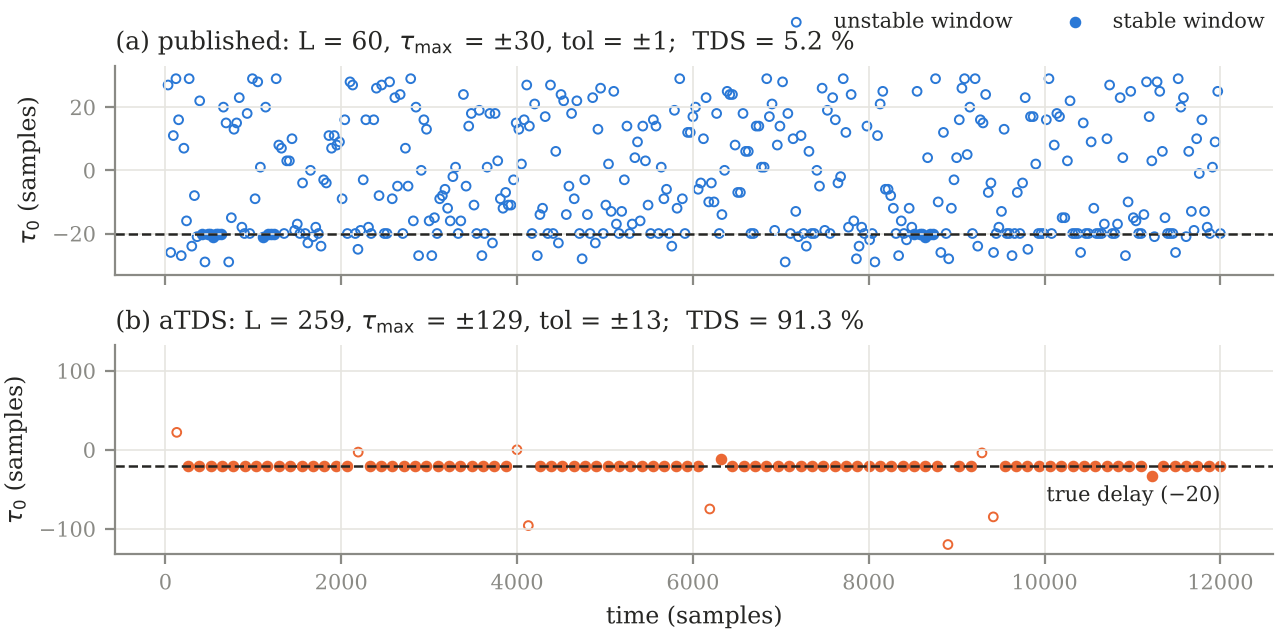
\includegraphics[width=\textwidth]{figures/fig_example_fixed_vs_atds.png}
\caption{The same coupled pair ($\tau_c = 8$, true delay 20 samples, coupling 0.6) under the published fixed parameters (a) and the parameters chosen by aTDS on a separate training pair (b). Each dot is $\tau_0$ in one window over the first 12\,000 samples; filled dots are stable windows. The dashed line is the true delay ($\tau = -20$; negative means $x$ leads).}
\label{fig:example}
\end{figure}

\subsection{Window}
\label{sec:res-window}
A fixed 60-sample window holds fewer independent samples the slower the signal, down to 0.93 at $\tau_c = 64$ (\cref{fig:window}a); the aTDS window holds 30 by construction. \Cref{fig:window}b varies only the window for two weakly coupled systems ($c = 0.3$): a faster one ($\tau_c = 4$, $d = 10$) and one four times slower ($\tau_c = 16$, $d = 40$), with $\tau_{\max} = (L-1)/2$ and the tolerance calibrated at every window length. aTDS chose 121 and 515 samples respectively, about four times longer for the four-times slower system, reaching AUC 0.97 [0.95, 0.99] and 0.79 [0.73, 0.85] against 0.83 and 0.51 at 60 samples. Detection keeps rising past the aTDS choice (0.99 at 1\,920 samples for the slower system): with coupling that is always on, a longer window is always better, so the aTDS window is a compromise with time resolution rather than the best window for detection.

\begin{figure}[t]
\centering
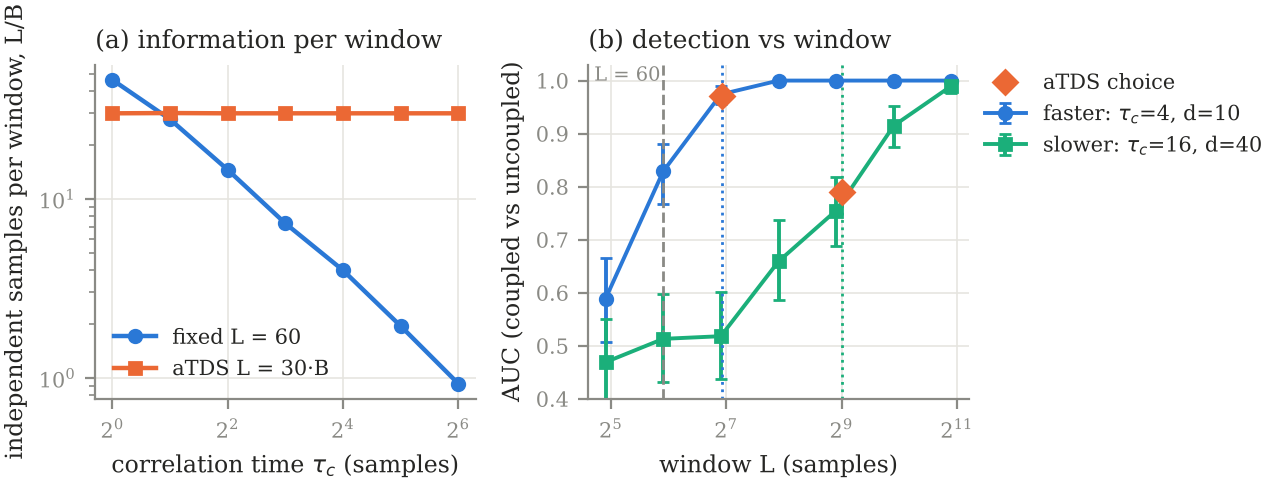
\includegraphics[width=\textwidth]{figures/fig_window_rule.png}
\caption{Window rule. (a) Independent samples per window, $L/B$, against the correlation time $\tau_c$ (median $B$ over 5 signals of 30\,000 samples). (b) AUC against window length for a faster and a four-times slower system with weak coupling (100 coupled and 100 uncoupled pairs per point; bootstrap 95\,\% intervals). Dotted lines and diamonds: the window chosen by aTDS for each system; dashed line: $L = 60$.}
\label{fig:window}
\end{figure}

To test the constant 30 when time resolution matters, coupling ($c = 0.6$, $\tau_c = 8$, $d = 20$) was switched on and off in blocks of 1\,000, 2\,000 or 4\,000 samples (40\,000 samples, 20 pairs per point). A window counts as correct if, during coupling, it is stable with $\tau_0$ within $\pm2$ samples of the true delay, or, without coupling, it is not stable. \Cref{fig:onoff} shows a real trade-off whose optimum depends on episode length: 45 independent samples for the shortest blocks (balanced accuracy 0.87; 30 gives 0.85), 60 for 2\,000-sample blocks (0.92; 30 gives 0.88), and a plateau of 0.94--0.95 from 45 on for the longest blocks (30 gives 0.91). The aTDS constant is within 0.015--0.05 of the best in all three cases, on the short side.

\begin{figure}[t]
\centering
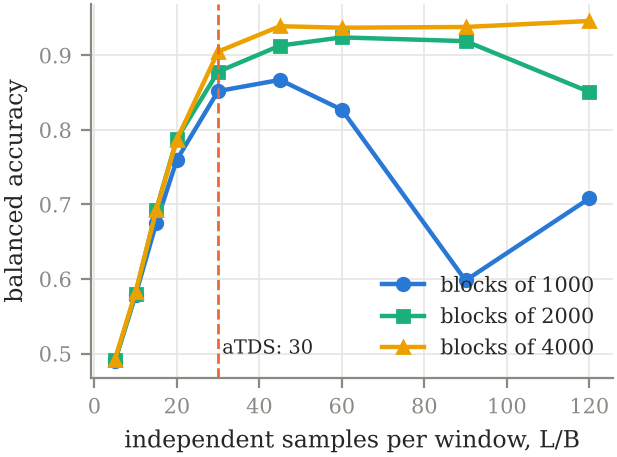
\includegraphics[width=0.55\textwidth]{figures/fig_onoff_tradeoff.png}
\caption{Coupling switched on and off in blocks of 1\,000--4\,000 samples. Balanced accuracy of the window labels against the number of independent samples per window; dashed line: the aTDS constant 30.}
\label{fig:onoff}
\end{figure}

\subsection{Lag range}
\Cref{fig:lag} isolates the lag range. Slow coupled signals ($\tau_c = 16$, $c = 0.6$) with true delays from 5 to 160 samples (10 pairs per delay) were scored with the aTDS window and tolerance (windows 454--514, tolerances $\pm23$ to $\pm29$) and either the published $\pm30$ or the aTDS range $(L-1)/2$ ($\pm226$ to $\pm256$). With the aTDS range the reported delay is exact for all 90 pairs, sign included. With $\pm30$, all 50 pairs with delays beyond 30 report a wrong delay at the edge of the search ($\pm30$, once 18), 16 of them with the wrong sign, while their TDS scores stay high (72--96\,\%). A high TDS score can therefore coexist with a wrong delay when the lag range is fixed. aTDS scores fall at long delays (27--62\,\% at $d = 160$) because the overlap of $x$ and delayed $y$ within a window shrinks; the delay reported from the stable windows remains right. Within $\pm30$ both variants are right and the narrow range scores somewhat higher (94--100\,\% vs 82--99\,\%), as it has fewer lags to pick wrongly by chance.

\begin{figure}[t]
\centering
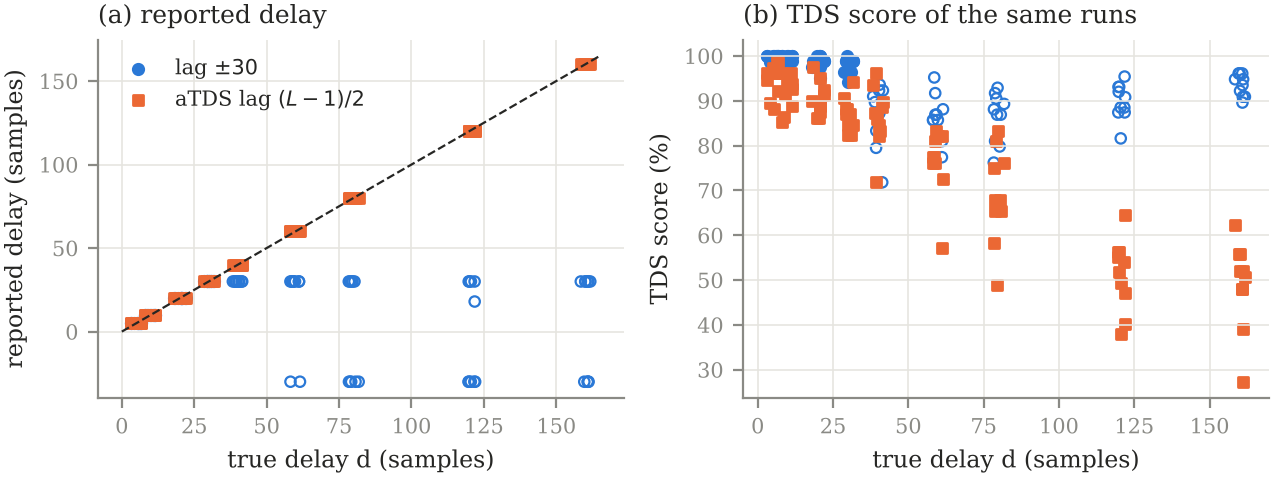
\includegraphics[width=\textwidth]{figures/fig_lag_range.png}
\caption{Only the lag range changes. (a) Reported delay ($-\tau_0$, with $\tau_0$ the most frequent value among stable windows; positive means $x$ leads) against the true delay; the dashed diagonal is a perfect answer. (b) TDS score of the same runs. Filled markers: right delay; hollow: wrong delay. Points are jittered horizontally.}
\label{fig:lag}
\end{figure}

\subsection{Tolerance}
\Cref{fig:tol}a shows the calibration on the example pair: the chance score of 20 rotated copies rises with the tolerance, and its upper bound crosses 5\,\% between $\pm12$ and $\pm13$; aTDS chose $\pm13$ from rotations of its training pairs. On the real pair (\cref{fig:tol}b) the score barely depends on the tolerance (90.0\,\% at 0, 91.3\,\% at $\pm13$), so the gain in \cref{fig:example} comes from the window and lag range. The tolerance caps false stability while allowing the delay to wobble.

\begin{figure}[t]
\centering
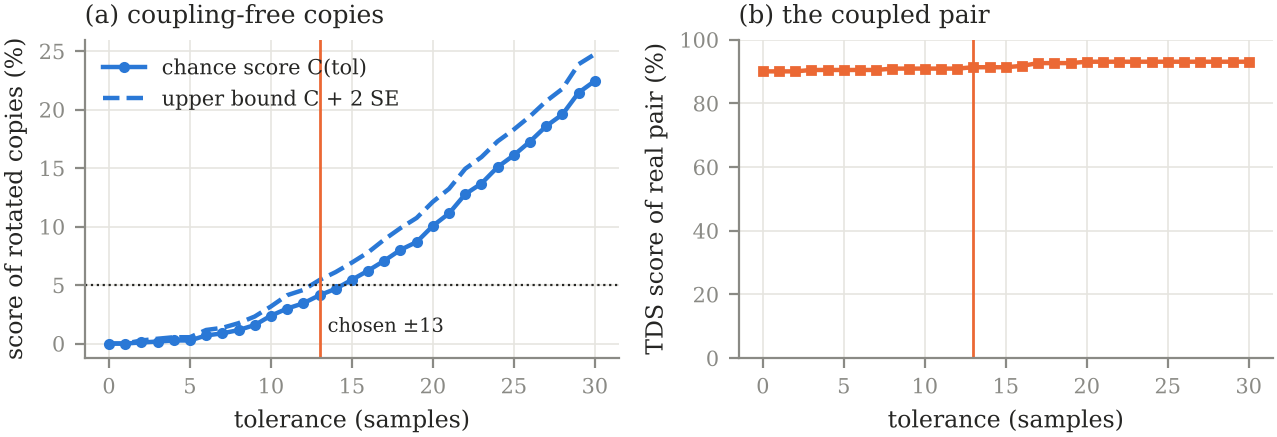
\includegraphics[width=\textwidth]{figures/fig_tolerance_calibration.png}
\caption{Tolerance calibration for the pair of \cref{fig:example} with the aTDS window. (a) Chance score $C(\mathrm{tol})$ of circularly rotated copies and its upper bound $C + 2\,\mathrm{SE}$; dotted line: 5\,\% budget. (b) TDS score of the real, unrotated pair at the same tolerances.}
\label{fig:tol}
\end{figure}

With the aTDS window and lag range fixed and only the tolerance changed ($\pm1$ vs calibrated; slow-down test, $c = 0.3$, 100 + 100 pairs per $r$), calibration helps slow systems recover the delay: 85\,\% vs 66\,\% of coupled pairs at $r = 8$ (intervals do not overlap), 88\,\% vs 77\,\% at $r = 4$ and 42\,\% vs 26\,\% at $r = 16$ (intervals overlap). The AUC gain ($+0.04$ at $r = 4$ and 8) is not significant at 95\,\%, and at $r = 1$ the calibrated tolerance is very slightly worse ($-0.005$, interval $-0.012$ to $-0.001$). The gain comes from having enough stable windows: with $\pm1$ only 77, 66 and 26 of 100 coupled pairs at $r = 4, 8, 16$ have 3 or more stable windows (almost all of them right), whereas with calibration 98, 93 and 53 have them, of which 90, 91 and 79\,\% are right. The mean chance score on new pairs is 3.3--4.4\,\% at every $r$, inside the budget.

\subsection{All three rules against fair baselines}
\Cref{fig:slowdown} and \cref{tab:slowdown} compare the four settings across the slow-down test. aTDS is far better than the published setting once the system is slower than that setting assumes (AUC 0.92 vs 0.59 at $r = 4$; 95\,\% interval of the difference $+0.24$ to $+0.42$); the published setting is close to chance from $r = 4$ on. Against the setting rescaled by hand, with a $\pm0.05$ equivalence margin, aTDS is equivalent at $r = 1$ and 2 (the rescaled setting is marginally higher at $r = 2$, 0.99 vs 0.98), better at $r = 8$ (0.88 vs 0.81; interval of the difference $+0.007$ to $+0.142$; delay found in 85\,\% vs 60\,\% of pairs) and undecided at $r = 4$ and 16 (90\,\% intervals $-0.064$ to $+0.003$ and $-0.105$ to $+0.018$). The oracle is better than aTDS at every $r \ge 2$, mostly by choosing much longer windows. The stricter v2.1 tolerance costs some detection at $r = 16$ (AUC 0.65, against 0.72 with an earlier rule and 0.69 for the rescaled setting).

\begin{figure}[t]
\centering
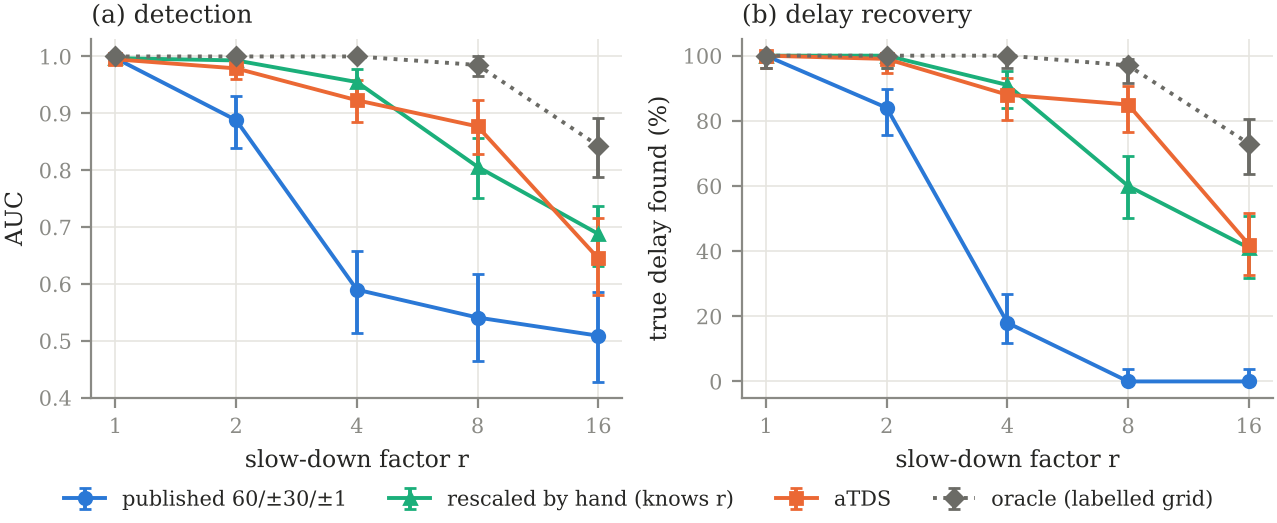
\includegraphics[width=\textwidth]{figures/fig_slowdown_baselines.png}
\caption{Slow-down test ($\tau_c = 2r$, $d = 5r$, coupling 0.3; 100 coupled and 100 uncoupled pairs per $r$). (a) AUC with bootstrap 95\,\% intervals. (b) Share of coupled pairs whose stable windows report the true delay, with Wilson 95\,\% intervals. The rescaled setting is given the true $r$; the oracle tunes on labelled pairs; aTDS is given neither.}
\label{fig:slowdown}
\end{figure}

\begin{table}[t]
\centering
\caption{Slow-down test: AUC [95\,\% interval] and parameters chosen. Window / lag / tolerance in samples.}
\label{tab:slowdown}
\resizebox{\textwidth}{!}{%
\begin{tabular}{rcccccc}
\toprule
$r$ & Published & Rescaled & aTDS & Oracle & aTDS parameters & Oracle parameters \\
\midrule
1  & 0.997 [0.989, 1.00] & 0.997 [0.989, 1.00] & 0.995 [0.988, 1.00] & 1.000 [0.999, 1.00] & 66 / 32 / 3     & 60 / 29 / 0 \\
2  & 0.888 [0.839, 0.93] & 0.993 [0.984, 1.00] & 0.979 [0.961, 0.99] & 1.000 [1.00, 1.00] & 126 / 62 / 6    & 240 / 119 / 0 \\
4  & 0.590 [0.513, 0.66] & 0.955 [0.926, 0.98] & 0.923 [0.885, 0.96] & 1.000 [1.00, 1.00] & 237 / 118 / 12  & 960 / 479 / 0 \\
8  & 0.541 [0.464, 0.62] & 0.806 [0.752, 0.86] & 0.877 [0.829, 0.92] & 0.985 [0.965, 1.00] & 563 / 281 / 27  & 1920 / 959 / 0 \\
16 & 0.509 [0.428, 0.59] & 0.688 [0.631, 0.74] & 0.645 [0.580, 0.72] & 0.843 [0.788, 0.89] & 1083 / 541 / 56 & 1920 / 959 / 135 \\
\bottomrule
\end{tabular}}
\end{table}

\subsection{Other signal classes and a real recording}
\Cref{tab:signals} runs aTDS against the published setting on signal classes typical of physiology. In every row aTDS set its parameters on data that were not scored. aTDS is better for strongly long-memory signals ($H = 0.9$), rhythms with delays below half a period, changing dynamics and Rulkov neurons, and equal or not distinguishable for $H = 0.6$ and 0.75. For a rhythm with a delay beyond half a period the coupling is detected but the delay is wrong, as expected from the lag cap. For a fast signal with a long delay (50 samples), the default lag range ($\pm30$) is too short and the optional $d_{\max}$ is needed. On the real EEG pair both settings detect the known strong coupling at delay 0; with no ground truth beyond detection, this row is counted neither for nor against aTDS.

\begin{table}[t]
\centering
\caption{Other signal classes (known answers) and one real recording. AUC with bootstrap 95\,\% intervals where available; ``found'': share of coupled pairs with the true delay.}
\label{tab:signals}
\footnotesize
\begin{tabularx}{\textwidth}{>{\raggedright\arraybackslash}p{3.4cm}>{\raggedright\arraybackslash}X>{\raggedright\arraybackslash}X>{\raggedright\arraybackslash}X}
\toprule
Signals & Published 60 / $\pm30$ / $\pm1$ & aTDS v2.1 & Reading \\
\midrule
fGn $H = 0.6$, $d = 20$, $c = 0.2$ & AUC 0.60 [0.47, 0.72], found 28\,\% & 0.59 [0.45, 0.71], 23\,\% ($L = 61$) & Equal \\
fGn $H = 0.75$, $d = 20$, $c = 0.2$ & 0.70 [0.59, 0.81], 33\,\% & 0.65 [0.53, 0.77], 23\,\% ($L = 73$) & Not distinguishable \\
fGn $H = 0.9$, $d = 20$, $c = 0.2$ & 0.46 [0.33, 0.58], 15\,\% & 0.82 [0.73, 0.91], 85\,\% ($L = 614$, $\pm34$) & aTDS better; $B$ grows with record length \\
Rhythm $P \approx 40$, $d = 8$ & 0.97, 43\,\% & 1.00, 100\,\% (period 41, lag $\pm20$) & aTDS better \\
Rhythm $P \approx 40$, $d = 30$ & 0.46, 0\,\% & 0.995, 0\,\% (reports 11) & Detected, delay wrong (anti-phase lobe) \\
Rulkov neurons, $d = 16$ / 32 & 0.73 / 0.79; median delay 0 / 15.5 & 1.00 / 1.00; median delay 19 / 35 & aTDS better; constant $+3$ offset \\
Fast ($\tau_c = 1$), $d = 50$, $c = 0.5$ & 0.56, 0\,\% & default ($L = 61$): 0.56, 0\,\%; with $d_{\max} = 60$ ($L = 121$): 1.00, 100\,\% & Needs optional $d_{\max}$ \\
Memory $\tau_c$ 4 $\to$ 16, $d = 10$, $c = 0.4$ & 1st half 0.98; 2nd half 0.71, 45\,\% & one window (252): 1.00 / 0.96, 90\,\%; per half (124 / 484): 1.00 / 0.98, 100\,\% & aTDS better; per segment slightly better \\
Mixed: slow ($\tau_c$ 32, $d = 40$) + fast ($\tau_c$ 2, $d = 5$) pair & slow 0.44, fast 1.00 & one window (972): 0.99 / 1.00, fast tol $\pm56$; per-pair: fast $L = 64$, $\pm3$ & System-wide window costs fast-pair precision \\
Slow $x$ ($\tau_c$ 32) drives fast $y$ ($\tau_c$ 2), $d = 10$ & 0.83, 57\,\% & max-$B$ window (939, $\pm51$): 1.00, 100\,\%; joint $B_{xy}$ (339, $\pm19$): 1.00, 100\,\% & Joint $B_{xy}$: same detection, 2.8$\times$ shorter window \\
Real sleep EEG $\delta$/$\sigma$ power, 1\,Hz (train 1st half, score 2nd) & 50.8\,\% vs chance 1.2\,\% & $L = 652$ (11 min), $\pm325$, $\pm22$: 95.5\,\% vs chance 2.1\,\% & Both detect, delay 0; not counted \\
\bottomrule
\end{tabularx}
\end{table}

Two rows point to refinements. In a mixed-speed network, a single window set by the slowest signal gives fast pairs a wide tolerance ($\pm56$ instead of $\pm3$ with a per-pair window). For a coupled fast--slow pair, the joint Bartlett factor $B_{xy} = 1 + 2\sum_k r_x(k)\, r_y(k)$ (11.3, between $B_x = 31.3$ and $B_y = 5.0$) gave the same detection with a window 2.8 times shorter and a tolerance 2.7 times tighter than the max-$B$ rule. For Rulkov neurons the delay was reported a constant 3 steps too long at both delays, probably the map's response latency; calibration did not fail under one-way coupling.

\subsection{Networks: per-link significance with FDR control}
\label{sec:res-network}
The 5\,\% budget bounds the mean chance score, not the false-positive rate of an individual link. For networks we therefore combine aTDS with a per-link rotation test: a link's $p$-value is $(1 + \#\{\text{rotations scoring} \ge \text{the real score}\}) / 1\,000$ over 999 rotations, and the 15 links of a six-signal network are tested together with the Benjamini--Hochberg procedure at $q = 0.05$~\cite{Benjamini1995ControllingFalse}. Two designs ($\tau_c = 8$, 10\,000 samples, coupling 0.4; 10 coupled and 10 uncoupled networks each) were tested: three disjoint links ($0\to1$, $2\to3$, $4\to5$; delays 10, 20, 15) and a common driver (0 drives 1 with delay 10 and 2 with delay 20, plus $3\to4$ with delay 15), which induces an indirect 1--2 link. aTDS set one parameter set per network by rotation only, without labels (tolerance calibrated on 4 rotations of each of the 15 pairs, 60 in total).

The per-link test was calibrated: on uncoupled links 2.7--5.8\,\% reached $p \le 0.05$. After FDR control no false link appeared in any of the 20 uncoupled networks. In the coupled networks aTDS found 27 of 30 true links (disjoint) and 26 of 30 (common driver), with a mean false-discovery proportion of 8.3\,\% and 2.5\,\%. With only 10 networks per design these proportions are imprecise, and the 8.3\,\% of the disjoint design, above the 5\,\% target, should be read as inconclusive rather than as a failure or a confirmation of FDR control. The indirect link of the common driver was not reported in any network (raw $p \le 0.05$ in 1 of 10); at coupling 0.4 the indirect correlation is only about $0.4 \times 0.4 = 0.16$. Pairwise TDS cannot distinguish indirect from direct links, so with stronger drivers indirect links are expected to appear.
%%%%%%%%% EXPERIMENTS %%%%%%%%%

\section{Discussion}
\label{sec:discussion}
%%%%%%%%% DISCUSSION %%%%%%%%%
aTDS does automatically what a careful analyst would do by hand: it scales the TDS parameters to the time scale of the system without being told that time scale. Its three rules address three distinct failure modes of a fixed setting. A window counted in samples carries less and less information as the system slows (\cref{fig:window}); a lag range counted in samples can exclude the true delay while still producing a high score (\cref{fig:lag}); and a tolerance of $\pm1$ is too strict for the natural wobble of a delay in slow systems, leaving too few stable windows to recover it. Against the published setting aTDS is much better whenever the system is slower than that setting assumes; against a hand-rescaled setting that is told the true slow-down factor, it is equivalent or better where the tests can decide.

\paragraph{Relation to the oracle.} The oracle chose long windows with tolerance 0 at $r = 2$--8 (\cref{tab:slowdown}), the opposite direction to the wider tolerances aTDS selects. The two are consistent: a longer window reduces the window-to-window jitter of $\tau_0$, so the delay can be held to a tight tolerance, whereas aTDS keeps the window at 30 independent samples for time resolution and compensates for the larger jitter with a wider, calibrated tolerance. At a fixed window, calibrating the tolerance improved delay recovery (85\,\% vs 66\,\% at $r = 8$); across windows, the oracle shows that users who do not need time resolution can gain detection by lengthening the window.

\paragraph{Biases of the null model.} Two simplifications of the rotation null act in the same direction. Rotating one signal removes slow co-modulation that both signals share, for example through sleep-stage changes; on such data the chance score is underestimated, the tolerance may be chosen too wide and per-link $p$-values are too small. The standard error in \cref{eq:tol} treats rotations as independent although rotations of one recording, and pairs that share a signal, are correlated; this underestimates the uncertainty of $C(t)$ and also favours a wider tolerance. On the synthetic data, which contain no shared co-modulation, the mean chance score on new data stayed within the budget in all but one case (5.2\,\%), but single recordings exceeded it by chance (95th percentile up to 20\,\%). For real staged data we therefore recommend the per-link test of \cref{sec:res-network} and, where cohorts are available, a cross-subject stage-matched null~\cite{Bashan2012NetworkPhysiology}.

\paragraph{Limitations.} aTDS is not optimal, only scaled: with permanent coupling, longer windows detect better, and the oracle outperforms aTDS at every $r \ge 2$. The 61-sample floor fixes a minimum lag range of $\pm30$, but delays beyond half the window remain out of reach without $d_{\max}$, and nothing in the output warns the user (for the fast signal with delay 50 the default score was 4.8\,\% against a chance score of 4.4\,\%); $d_{\max}$ was tested only with a correct value. In records shorter than about 600 samples the floor exceeds the 10\,\% cap, leaving fewer than 19 windows. Longer windows mean one answer per longer span (11 minutes on the EEG pair), so short coupling episodes can be missed; a maximum window or per-segment calibration trades reliability for time resolution. The calibrated tolerance grows with the time scale (up to $\pm56$ at $r = 16$) and can exceed the delay itself, so the stability judgement is coarse even when the reported delay is right. The 5\,\% budget concerns the mean: with pooled rotations and the upper-bound rule the mean chance score on new data stayed $\le 5\,\%$ in all rows but one (5.2\,\%, fast--slow pair with the max-$B$ window), while single recordings still exceed it by luck (95th percentile up to 20\,\%), hence the per-link test. For long-memory signals $B$ depends on record length ($H = 0.9$: 13 to 84 for 5\,000 to 80\,000 samples). Rhythmic and bursting signals are best converted to cycle-by-cycle series first. Finally, aTDS scores are not comparable with published TDS scores; an aTDS score should be compared with the aTDS chance level of the same data. The design constants other than the number of independent samples per window (the 5\,\% budget, the 61-sample floor, 20 rotations per pair and the 2-SE margin) were not varied in our tests, and per-link detection power was measured only in the network test; the slow-down comparison uses AUC across pairs.

\subsection*{Practical guidance}
\label{sec:guidance}
\begin{itemize}
\item \textbf{Report} each aTDS score together with the aTDS chance level of the same data and the chosen parameters $(L, \tau_{\max}, \mathrm{tol})$; for networks, report per-link $p$-values from rotations with FDR control rather than thresholded scores.
\item \textbf{Long delays in fast signals:} if a delay longer than about 30 samples is plausible, supply $d_{\max}$; without it such a delay is out of reach and the score looks like no coupling (4.8\,\% vs a chance level of 4.4\,\% in our test, against AUC 1.00 with $d_{\max}$). A pile-up of $\tau_0$ values at $\pm\tau_{\max}$ is a warning sign that the delay lies outside the lag range; reporting the share of stable windows whose $\tau_0$ lies at the edge of the lag range could serve as an automatic check, but this is untested and would not flag our fast-signal case, whose score was at chance level and so had almost no stable windows.
\item \textbf{Pairs of very different speed:} consider the joint factor $B_{xy}$ for the window of that pair (one configuration tested, both rules at AUC 1.00; weaker coupling untested).
\item \textbf{Time resolution:} if the chosen window is too long for the question (11 minutes on the EEG pair), cap it; capping at 300\,s kept the EEG coupling clearly detectable (82.7\,\% vs a chance level of 2.3\,\%). Even a 300-s window spans ten 30-s scoring epochs, so aTDS, like TDS with any window of this length, describes coupling over several epochs rather than within a single one. For records whose dynamics change, set the parameters per segment.
\item \textbf{Rhythmic and bursting signals:} convert them to cycle-by-cycle series first; otherwise delays beyond half a period are reported as the anti-phase lobe.
\end{itemize}

\begin{table}[t]
\centering
\caption{Summary of the evidence. AUC differences are aTDS minus the comparison, with 95\,\% intervals.}
\label{tab:summary}
\footnotesize
\begin{tabularx}{\textwidth}{>{\raggedright\arraybackslash}p{4.2cm}>{\raggedright\arraybackslash}X}
\toprule
Comparison & Result \\
\midrule
aTDS vs published 60 / $\pm30$ / $\pm1$ (\cref{fig:slowdown}) & Better from $r = 2$ on ($+0.05$ to $+0.14$ at $r = 2$; $+0.24$ to $+0.42$ at $r = 4$; $+0.03$ to $+0.25$ at $r = 16$); equal at $r = 1$. \\
aTDS vs rescaled by hand (\cref{fig:slowdown}) & Equivalent ($\pm0.05$ AUC) at $r = 1, 2$; better at $r = 8$; undecided at $r = 4, 16$. aTDS is not told $r$. \\
aTDS vs oracle grid & Oracle better at $r \ge 2$, mostly through longer windows. \\
Lag range only (\cref{fig:lag}) & $\pm30$: wrong delay for all 50 pairs with delays beyond 30 (16 with the wrong sign) at scores of 72--96\,\%; aTDS exact in all 90 pairs. \\
Tolerance only & Delay found more often at $r = 8$ (85 vs 66\,\%); higher at $r = 4, 16$ (not significant); AUC gain not significant; chance 3.3--4.4\,\%. \\
Window and on/off coupling (\cref{fig:onoff}) & 30 independent samples within 0.015--0.05 of the best balanced accuracy, on the short side. \\
Other signals (\cref{tab:signals}) & Better on $H = 0.9$, rhythms with delay below half a period, changing dynamics and Rulkov detection; equal on $H = 0.6, 0.75$; wrong delay beyond half a period; long delay in a fast signal needs $d_{\max}$. \\
Networks (\cref{sec:res-network}) & 0 false links in 20 uncoupled networks; 87--90\,\% of true links found; FDP 2.5--8.3\,\%. \\
\bottomrule
\end{tabularx}
\end{table}

\paragraph{Not tested.} No test switches the coupling itself on in one physiological regime and off in another, which is the sleep-stage case; whether parameters should be set per stage or frozen per cohort, and how that changes stage contrasts, requires staged multi-subject recordings. The rotation null used here removes stage-driven co-modulation that the cross-subject, stage-matched null of Bashan et al.\ keeps, so it may be too lenient on real data. Rotations of one recording are not independent; a standard error clustered by recording would be more conservative.

\paragraph{Next steps.} (i) Apply aTDS to a public staged sleep cohort, with cross-subject, stage-matched surrogates next to the rotation null. (ii) Adopt the joint $B_{xy}$ as the window rule for pairs of different speed and repeat the tests. (iii) Test networks with stronger common drivers and chains, and whether partial (conditional) TDS is needed. (iv) Add a regime-switching benchmark in which the coupling itself turns on and off. (v) Use a recording-clustered standard error in the tolerance rule and report per-link power in the slow-down setting.
%%%%%%%%% DISCUSSION %%%%%%%%%

\section{Conclusion}
\label{sec:conclusion}
%%%%%%%%% CONCLUSION %%%%%%%%%
Time Delay Stability depends on three parameters counted in samples whose published values fit one kind of data. aTDS replaces them by rules based on each signal's own autocorrelation and on coupling-free rotated copies: a window of 30 independent samples, a lag range of half the window, and a tolerance set by a 5\,\% false-stability budget. On synthetic signals with known answers it is equivalent to or better than a hand-rescaled setting where the tests can decide ($r = 1, 2, 8$), and undecided elsewhere, without being told the time scale, removes a silent failure in which a fixed lag range reports wrong delays at high scores, and, combined with a per-link rotation test and FDR control, produced no false links in uncoupled networks. Its value lies in automation with a false-alarm budget; whether it sharpens physiological network contrasts in real sleep cohorts is the next question to answer.
%%%%%%%%% CONCLUSION %%%%%%%%%

\section*{Code and data availability}
pyTDS, the aTDS experiment scripts, their raw results (JSON) and the figure scripts are available at \url{https://github.com/Marku-a/pyTDS}. All random seeds are fixed.

\section*{Use of AI tools}
This manuscript was drafted with the PaperOrchestra multi-agent writing pipeline, with a large language model as its backbone, from the author's method description, experiment scripts and raw results. All numbers were checked against the raw results. The experiments and an earlier technical report were reviewed by an AI model acting as a referee; the work has not yet been reviewed by a human expert.

%%%%%%%%% REFERENCES %%%%%%%%%
\bibliographystyle{unsrtnat}
\bibliography{references}
%%%%%%%%% REFERENCES %%%%%%%%%

%%%%%%%%% Appendix %%%%%%%%%
% If you want to add appendix, uncomment the following lines:
% \appendix
% \section{xxx}
%%%%%%%%% Appendix %%%%%%%%%

\end{document}